\chapter{Introduction to Organisation}\hrule
\label{Chapter:1}
% =====================================================================================================
\section {Organisation Profile and History}

I had my Six Months Training at Auribises Technologies, Ludhiana. Auribises Technologies was founded in Nov, 2011 by Mr. Ishant and some of its colleagues. The company has great fame in training students in Andriod, Java EE, AI, Java SE, Web related technologies across India. It is an ISO 9001-2015 certified company.
\\
\\
The company main motive is to impart the deep programing and computing skills in the students across india in an affordable way. The company also provides online training on various skills like Data Science. It also have experience in training employees of various big corporate IT firms across india.\\
\\
The Institute is at 4 Km driving distance from Ludhiana Junction, located in Krishna Nagar, Ludhiana, Punjab.It is an ISO 9001:2008 certified company. The company has a well equipped lab facility available for its students.
\\
\\
Auribises was founded in 2011 in Ludhiana (India) by Ishant Kumar and has been very successful in the field of software development and IT Training ever since.The core competency of Auribises is the development of software solutions for common problems of users, developers and enterprises. As an IT service provider Auribises develops individual desktop, server, web-based, mobile-based software solutions as requested by the cutomer.
\\
\\
Auribises is a leading technical service provider. Their goal is to be the leading independent provider of technical services for development, consultation and training. Since 2011, They have been developing solutions to ensure the quality and economic efficiency. They firmly believe that social and technological progress is inextricably linked together and implementing the combination Auribises aims to deliver "end user happiness".
\\
\\
Two words that perfectly encapsulate their commitment to service: whatever they do, they do it precisely and they do it right. They use new ideas, technology and expertise for development of products, services, systems and people and make them more competitive. Their Training Services are based on latest technologies which inspire their customers. Team Auribises create optimal software solutions and guarantee high-quality customer support.
\\
\\
The institute has more than 1K students who are trained in various latest software technologies in a year. The company has excellent history in software training and the company is also keenly looking forward to continue its legacy.

\chapter{Introduction to Project}\hrule
\label{Chapter:2}
% =====================================================================================================
\section{Overview}

Scisso App aims to solve problems of the Salon Managment and marketing across the country. The main motive of Scisso App is keeping the retention rate of the customers as high as possible by providing offers and loyalty points to the user for each purchase they make. This app will help Salon Admin to keep track of their product delivery, customer retention and Employee efficiency.\\
\\
While developing the project, i followed the industry standards of MVC i.e Model View Controller model. It follows the software engineering principles of low coupling and high cohesion. This model is followed to develop better softwares and to maintain a sustianable software product for a longer period of time.\\
\\
\textbf{What is MVC model?}\\
The MVC pattern allows separate the Controller layer from the logic, so that everything about how the interface works is separated from how we represent it on screen. \\
\\
Ideally the MVC pattern would achieve that same logic might have completely different and interchangeable views.\\
\\
\textbf{Why use MVC?}\\
In Android we have a problem arising from the fact that Android activities are closely coupled to both interface and data access mechanisms. We can find extreme examples such as Adapters, which are part of the view, with cursors, something that should be relegated to the depths of data access layer .

For an application to be easily extensible and maintainable we need to define well separated layers. What do we do tomorrow if, instead of retrieving the same data from a database, we need to do it from a web service? We would have to redo our entire view .

MVC makes views independent from our data source. We divide the application into at least three different layers, which let us test them independently. With MVC we are able to take most of logic out from the activities so that we can test it without using instrumentation tests.\\

While developing the project the main focus was that how the app will keep track of its customers and their transactions. Different API and their standard methods has been used to ensure that the app works superbly. Different latest android concepts like CardView also have been used in the project in order to have it a beautiful UI.\\
\\
The app is a total solution for the managment and marketing of a Slaon. The app allows the admin to handle the services provoided by them. The services are arranged according to the their categories. Along with services admin is allowed to handle and edit the data of their clients. Along with these facilities app also saves and have track of the employees working in the salon. Along with all these app also counts the incentives gained by the employees. These modules were from the sofware solutions that are provided by the app. The app also provide the Salon with marketing solution by rolling offers and by giving loyalty points on every purchase a customer make. 
\\

The app has a Main Activity which opens up a navigation menu and list of enabled services and current offers. The offers menu is developed in according to the customer view.
On the other hand the Navigation view is developed for the admin.
\\
\\
The Services nav item will lead the app to Services Activity where the admin can customize the services provided by them.
\\
\\
The Employees nav item intent the app to the Emploee List Activity where the admin can manage the details of the employees working in the salon.
\\
\\
The Clients nav item takes the app to Clients List Activity where the admin is allowed to perform the CRUD operations on the client and fix appointment with them.
\\
\\
The Appointements booked can be seen in by Appointments nav item.
\\
\\
The Offers nav item is for managing the offers rolling in the Salon at the current time.
\\
\\
The Redeem points module is mainly focused on the marketing sloutions of the salon. With the enough loyalty points collected a customer can get any of the current offers.
\\
\\
The Employee Accounts is for the calculation of the amount of work done by an employee in a given time.
\\
\\
Genrate receipt module generates the receipt for the services taken by a client.
\\
\\

Future of the app is to bring all the data of every salon using the app at a single database which will contain the data of all the clients from all the salon's and after gathering all the data we can analyse them and run acccording ads to the particular customer.

\section{Existing System}
No such type of Independent App exists for the Salon app managment which can provide both of the Software and marketing solutions. Though there are some of the apps like Vaniday which are providing great software soltions to the Salon's.


\subsection{Requirements Gathering}
Requirements gathering is also popularly known as requirements elicitation. The primary objective of the requirement gathering task is to collect the requirements from the stakeholders.\\
A stakeholder is a source of requirements and is usually a person, or a group of persons who either directly or indirectly are concerned with the software.\\
\\
Procedures adopted while requirements gathering during the project were:
\begin{itemize}
	\item \textbf{Interview:} A team of Fusion Salon, Ludhiana delivered the requirements to the Auribises Developers team.
	\item \textbf{Scenerio Amalysis:} The different use cases and functionality of the app were discussed. It includes the discussion on Main panel and followed by transaction history for a Salon.
	\item \textbf{Task Analysis:} The technologies to be used in Frontend and Backend were discussed.
	\item \textbf{Studying Documentation}: The documentation of various cloud technologies were studied and discussed with the Project Mentor. Finally, we agreed on using \textbf{Google Firebase} and \textbf{Google Cloud Platform} as our cloud technology.
\end{itemize}
\subsection{Functional Requirements}
\begin{itemize}
	\item Salon Admin need an Android phone with good internet connection.
	\item Android phone needs to have atleast 1 GB Ram and atleast 2GB of external usable memory.
	\item Android phone should have android os version "Kit-Kat" or above.
\end{itemize}
\section{Feasibility Study}
A feasibility study is used to determine the viability of an idea, such as ensuring a project is legally and technically feasible as well as economically justifiable. It tells us whether a project is worth the investment—in some cases, a project may not be do-able. There can be many reasons for this, including requiring too many resources, which not only prevents those resources from performing other tasks but also may cost more than an organization would earn back by taking on a project that isn’t profitable.\\
\\
The application is fully feasible. It just needs a working internet connection and android 4.0 and above. It is fully feasible if it is also deployed on a large scale.\\
The application can also be upgraded further and can be deployed on large scale depending upon the need of business plan.\\
\begin{enumerate}
	\item \textbf{Technical Feasibility :} The app is fully feasible on technical terms. I have android studio and required 8 GB Ram for development purpose.\\
	I will use Firebase cloud to deploy backend as it is free for inital and small projects.\\
	The version control system is completely free and the website Github.com is also free for Open Source Projects.
   \item \textbf{Economic Feasibility :} The app is fully economically feasible as it has free and open source tools being used while developing the system.\\
   The Firebase Cloud technology is free till 10K hits in a day. So, intially around 6-7 months after releasing the project, it is expected to have a user base of around 10K people. Later on, If the user base increases, the revenue of product will also increase and further resources can be purchased.
   \item \textbf{Legal Feasibility :} The app doesn't violates any legal rights and will credit the author of open Source Library used while developing the project.\\
   The project will be available in open source under \textbf{GPLv3} license.\\
   \\
   \textbf{What is GPLv3 License?}
   \begin{itemize}
   	\item The source code must be made public whenever a distribution of the software is made.
   	\item Modifications of the software must be released under the same license.
   	\item Changes made to the source code must be documented.
   	\item If patented material was used in the creation of the software, it grants the right for users to use it. If the user sues anyone over the use of the patented material, they lose the right to use the software.\\
   \end{itemize}
 
   \item \textbf{Operational Feasibility : } As the app satisfies the functional and non functional requirements, the app will be fully operational once it releases.
   
   \item \textbf{Scheduling Feasibility : } The project release targets for different versions are practical and have plenty of time develop and debug the app before release.
\end{enumerate}

\section{Objectives of the Project }
\begin{itemize}
	\item The project is developed to give a software solution and a marketing solution to the Salon Admin.
	\item The main motive behind developing the project is to rescue the Salon from hectic calculations. The app will help Salon to increase their revenue.
	\item This app will provide us with a large database of the customers which can be used to analyse and run ads accordingly.
\end{itemize}


\chapter{Product Design}\hrule
\label{Chapter:3}
% =====================================================================================================

\section{Product Perspective}
The application will have a user friendly and menu based interface. Till now, these activities are added.
\begin{itemize}
	\item A Splash Screen
	\item A Login Screen.
	\item A Main Screen.
	\item A Services Menu Screen.
	\item An Offers Menu Screen.
	
	\item An enabled services category list.
	\item A disabled services category list.
	\item An enabled services list.
	\item A disabled services list.
	
	\item An enabled employees list.
	\item A disabled employees list.

	
\end{itemize}
\section{Product Functions}
\begin{itemize}
	\item Salon Admin can handle Services provided in the salon.
	\item Salon Admin can handle Employees.
	\item Salon Admin can add Clients and handle them.
	\item Salon Admin can add and disable offers of the Salon.
	\item Salon Admin can view Emplyee Account details for a specific data range.
	\item Salon Admin can add Appointments for a client.
	\item Salon Admin can view the Appointments according to a specific date.
	\item Salon Admin needs to click Logout options menu to Logout from the app.
\end{itemize}

\section{Constraints} 
\begin{itemize}
	\item Admin needs Android 4.4 i.e "KitKat" and above.
	\item Admin needs active internet connection.
	\item Admin need to set the incentive and loyalty points percentage.
\end{itemize}

ScissoReport
\section{Database Design}
The database is a NoSQL Database. The data is stored in Tree data structure.\\
\subsection{NoSQL Database}
\textbf{What is NoSql Database?}\\
\\
NoSQL is an approach to database design that can accomodate a wide variety of data models, including key-value, document, columnar and graph formats. NoSQL, which stand for "not only SQL," is an alternative to traditional relational databases in which data is placed in tables and data schema is carefully designed before the database is built. NoSQL databases are especially useful for working with large sets of distributed data.\\

\section{Assumptions and Dependencies}
\begin{itemize}
	\item Admin is assumed to be using Android 4.4 and above.
	\item Admin is assumed to have working internet connection.
	\item Incentives and loyalty points are dependent on the respective rate.
	\item Date is dependent on system time. 

\end{itemize}
\section{Specific Requirements}
\begin{itemize}
	\item Android 4.4 and above.
	\item Working internet connection.
	\item Minimum 1 GB Ram and 2 GB external memory.
\end{itemize}
\chapter{Development and Implementation}\hrule
\label{Chapter:4}
% =====================================================================================================
\section{Introduction to Languages}
\subsection{Front End}
\textbf{XML}\\
XML is used as to design beautiful UI to give user a beautiful experience. Now a days, an app business is more dependent on how interactive, beautiful and simple your UI is.\\

XML data is known as self-describing or self-defining, meaning that the structure of the data is embedded with the data, thus when the data arrives there is no need to pre-build the structure to store the data; it is dynamically understood within the XML. The XML format can be used by any individual or group of individuals or companies that want to share information in a consistent way. XML is actually a simpler and easier-to-use subset of the Standard Generalized Markup Language (SGML), which is the standard to create a document structure.\\
The basic building block of an XML document is an element, defined by tags. An element has a beginning and an ending tag. All elements in an XML document are contained in an outermost element known as the root element. XML can also support nested elements, or elements within elements. This ability allows XML to support hierarchical structures. Element names describe the content of the element, and the structure describes the relationship between the elements.\\
An XML document is considered to be "well formed" (that is, able to be read and understood by an XML parser) if its format complies with the XML specification, if it is properly marked up, and if elements are properly nested. XML also supports the ability to define attributes for elements and describe characteristics of the elements in the beginning tag of an element.\\

\textbf{Java}\\
In the back end,JAVA is used. Collection and Genrics concepts are mainly used. Java is one of the world's most important and widely used computer languages, and it has held this distinction for many years. Unlike some other computer languages whose influence has weared with passage of time, while Java's has grown.\\

As of 2016, Java is one of the most popular programming languages in use, particularly for client-server web applications, with a reported 11 million developers using and working on it.\\
Applications of java:\\
Java is widely used in every corner of world and of human life. Java is not only used in softwares but is also widely used in designing hardware controlling software components. There are more than 930 million JRE downloads each year and 3 billion mobile phones run java.\\

Following are some other usage of Java :
\begin{itemize}
	\item Developing Desktop Applications.
	\item Web Applications like Linkedin.com, Snapdeal.com etc.
	\item	Mobile Operating System like Android.
	\item	Embedded Systems.
\end{itemize}

\textbf{Android Platform}\\
The Android platform is an open source mobile development platform. It gives you access to all aspects of the mobile device that it runs on, from low level graphics, to hardware like the camera on a phone. With so many things possible using Android, you might wonder why you need to bother with XML. It is not that working with XML is so interesting, it is working with the things that it enables. XML is commonly used as a data format on the Internet. If you want to access data from the Internet, chances are that the data will be in the form of XML. If you want to send data to a Web service, you might also need to send XML. In short, if your Android application will leverage the Internet, then you will probably need to work with XML. Luckily, you have a lot of options available for working with XML on Android.

\subsection{Back End}
\textbf{Firebase}\\
Web and mobile application often require back-end code to execute tasks like: sending out notifications or processing long running tasks (e.g. scaling images etc). In the traditional approach this back-end code is running on a server.\\
Recently Google’s Firebase introduces a new functionality which is called Cloud Functions. With this new service Firebase offers a scaleable solution for running back-end code in the cloud. Running code in the cloud has various advantages:
\begin{itemize}
	\item You do not need to run and maintain your own server.
	\item You do have an isolated code base for back-end code.
	\item You only get billed for the actual executing time of you code.
\end{itemize}
\pagebreak
\section{Implementation with ScreenShots}

\begin{figure}[h]
	\centering
	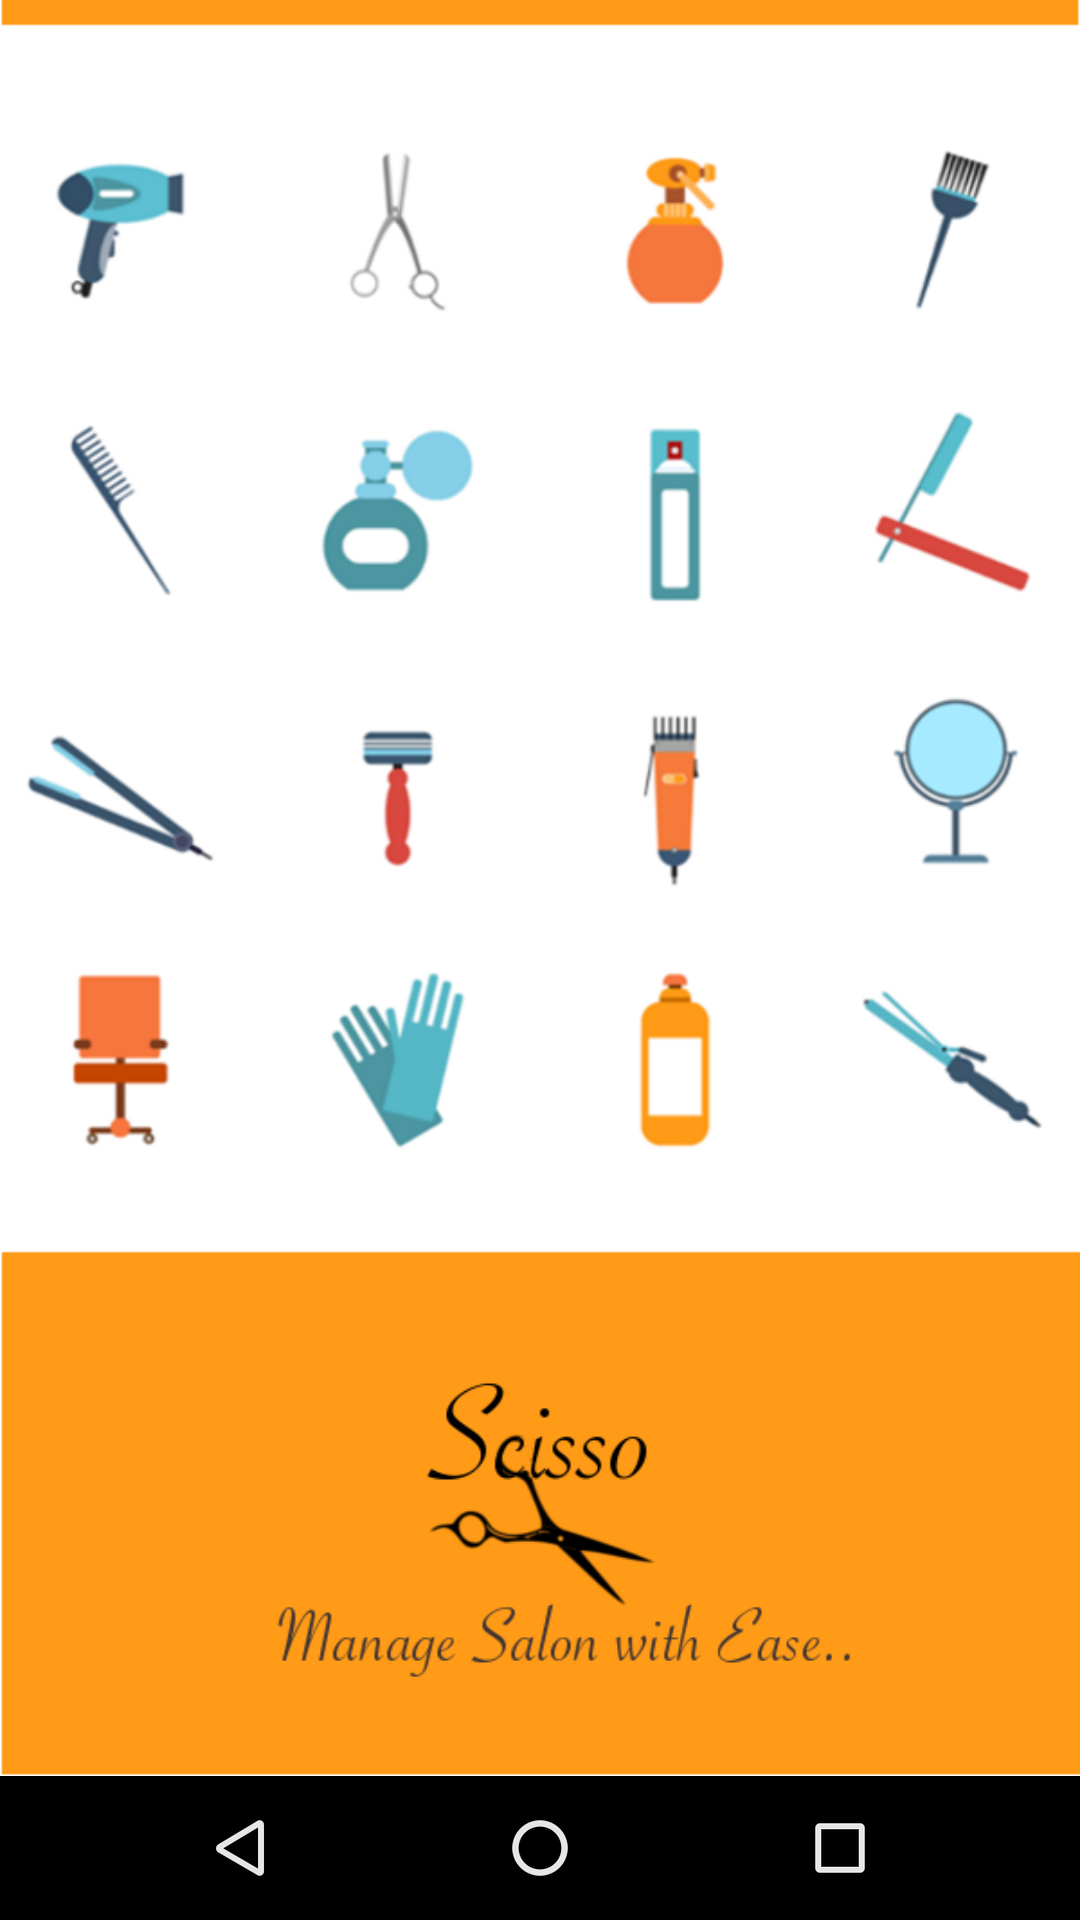
\includegraphics[width=0.7\linewidth]{SplashYes}
	\caption{Splash Screen}
\end{figure}
\pagebreak

\begin{figure}[h]
	\centering
	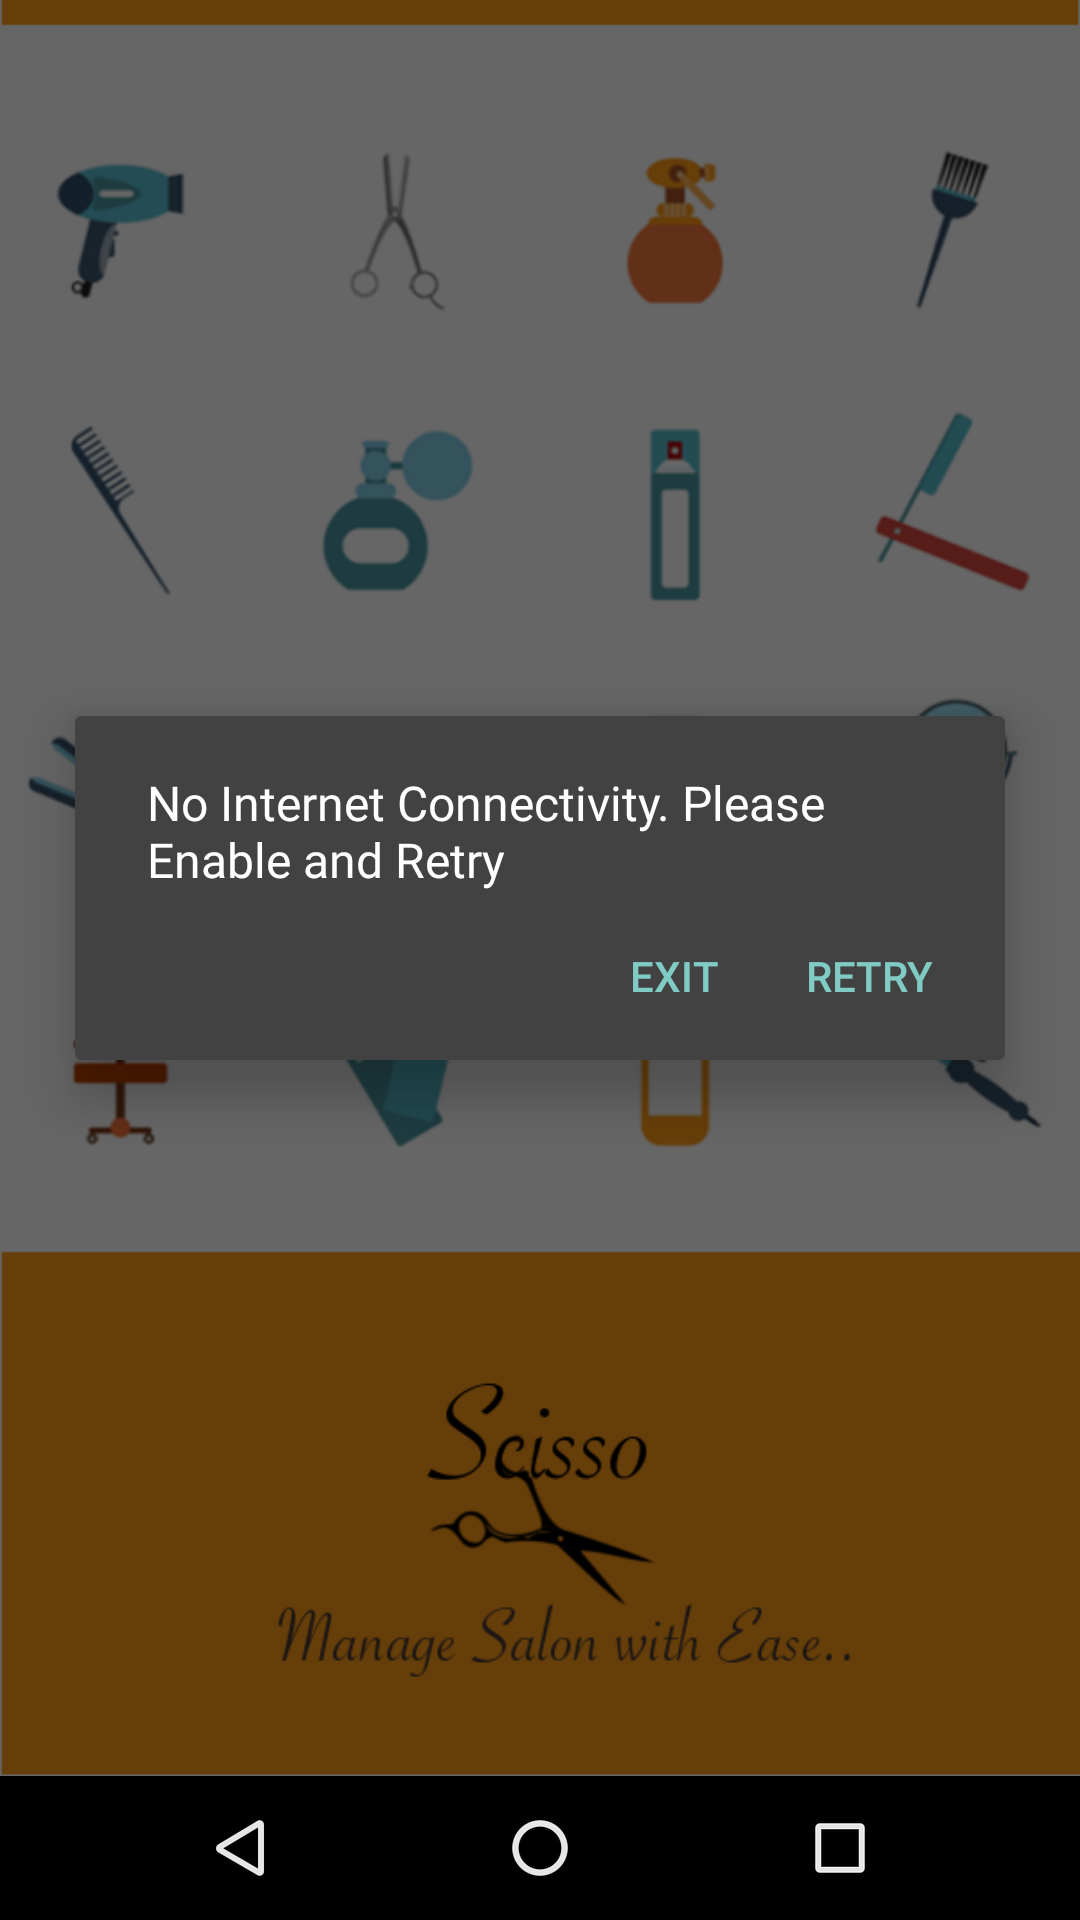
\includegraphics[width=0.7\linewidth]{SplashNo}
	\caption{Disconnected Dialog}
\end{figure}
\pagebreak

\begin{figure}[h]
	\centering
	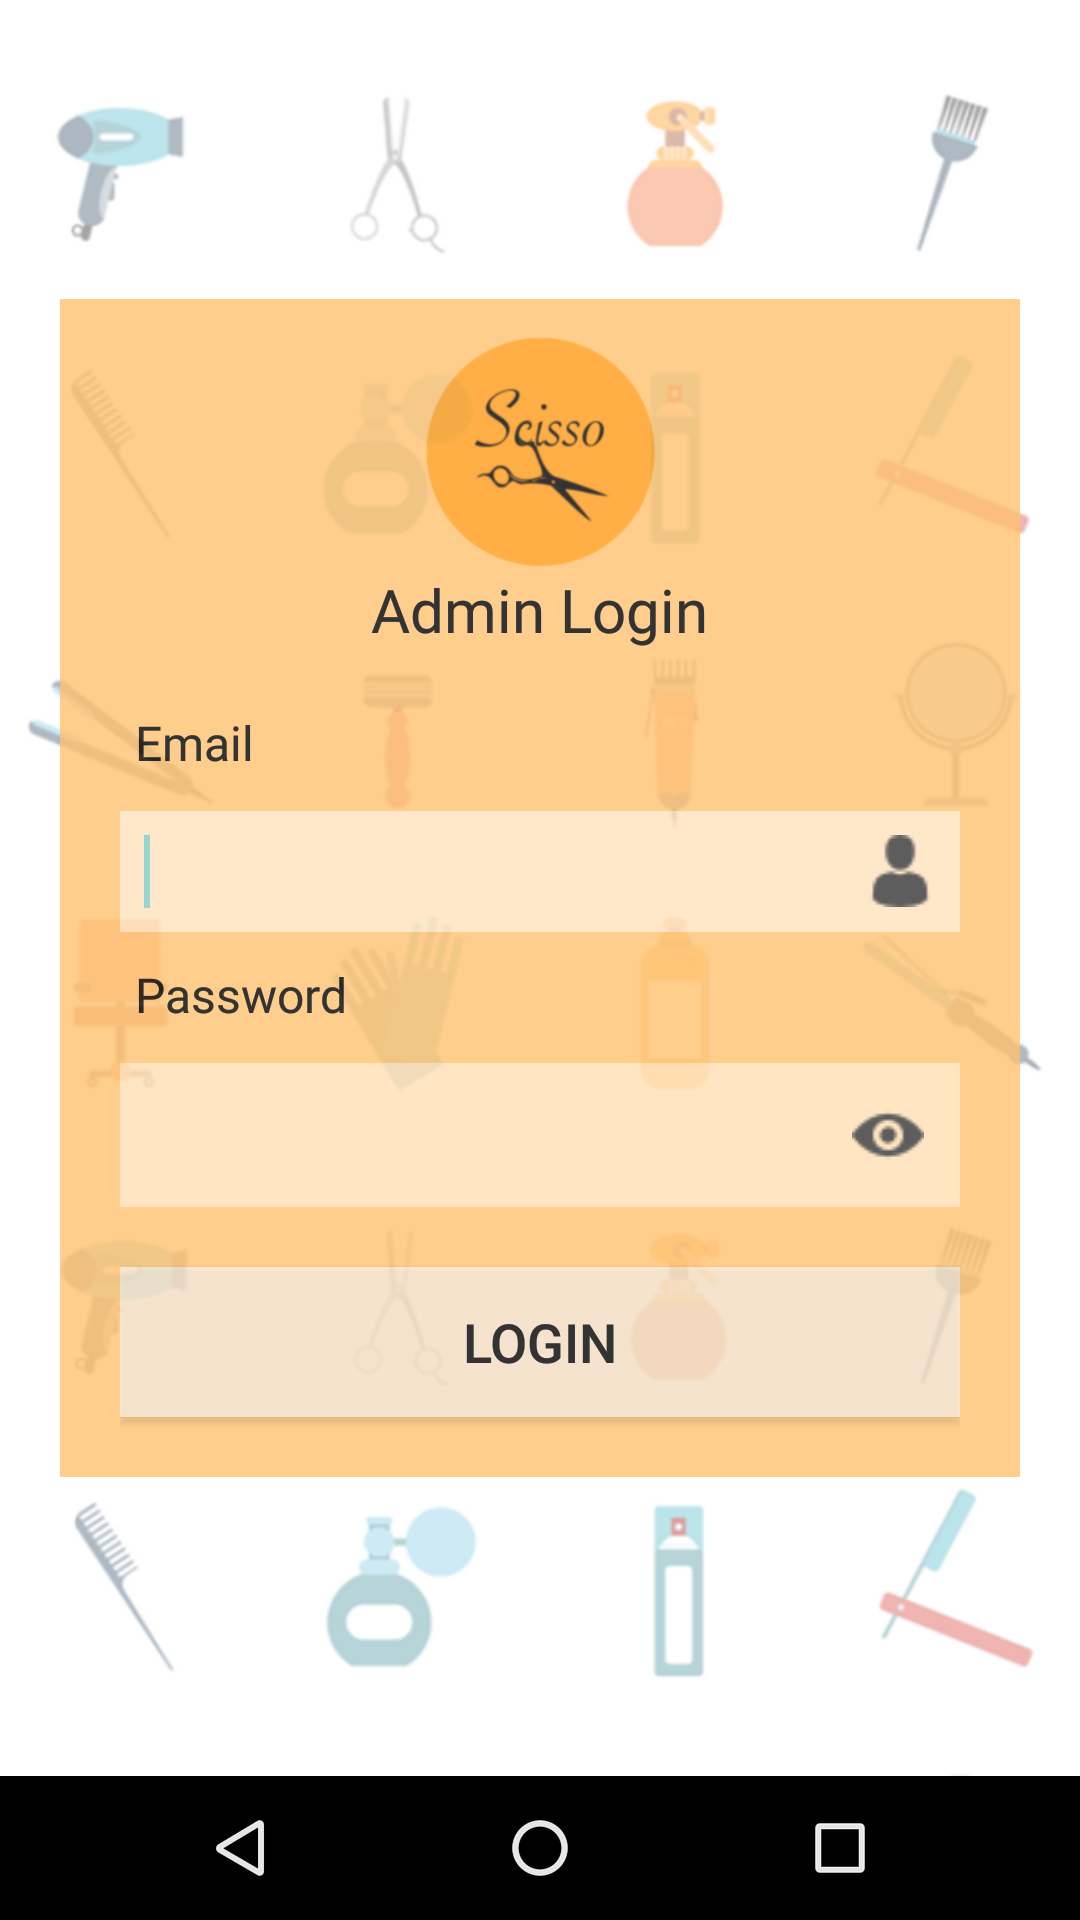
\includegraphics[width=0.7\linewidth]{LoginScreen}
	\caption{Login Screen}
\end{figure}
\pagebreak

\begin{figure}[h]
	\centering
	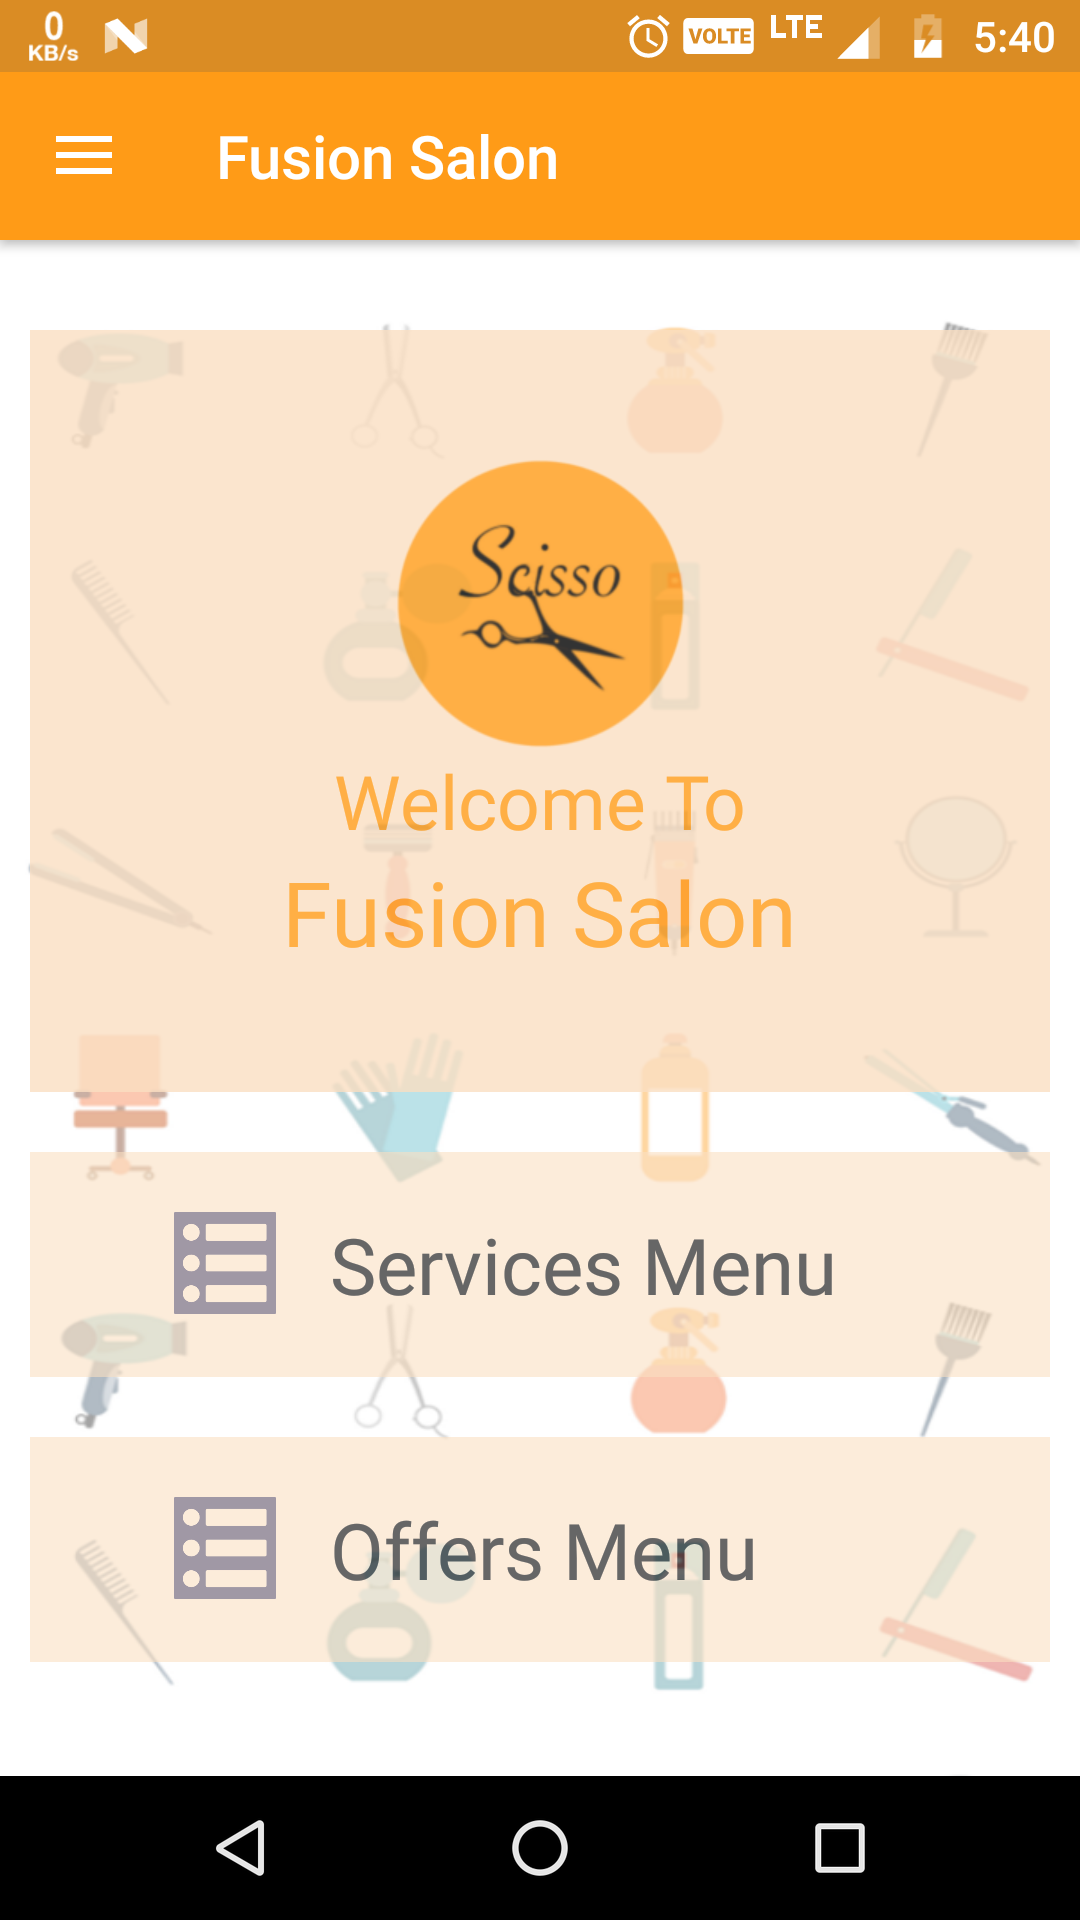
\includegraphics[width=0.7\linewidth]{MainActivity}
	\caption{Main Activity}
\end{figure}
\pagebreak

\begin{figure}[h]
	\centering
	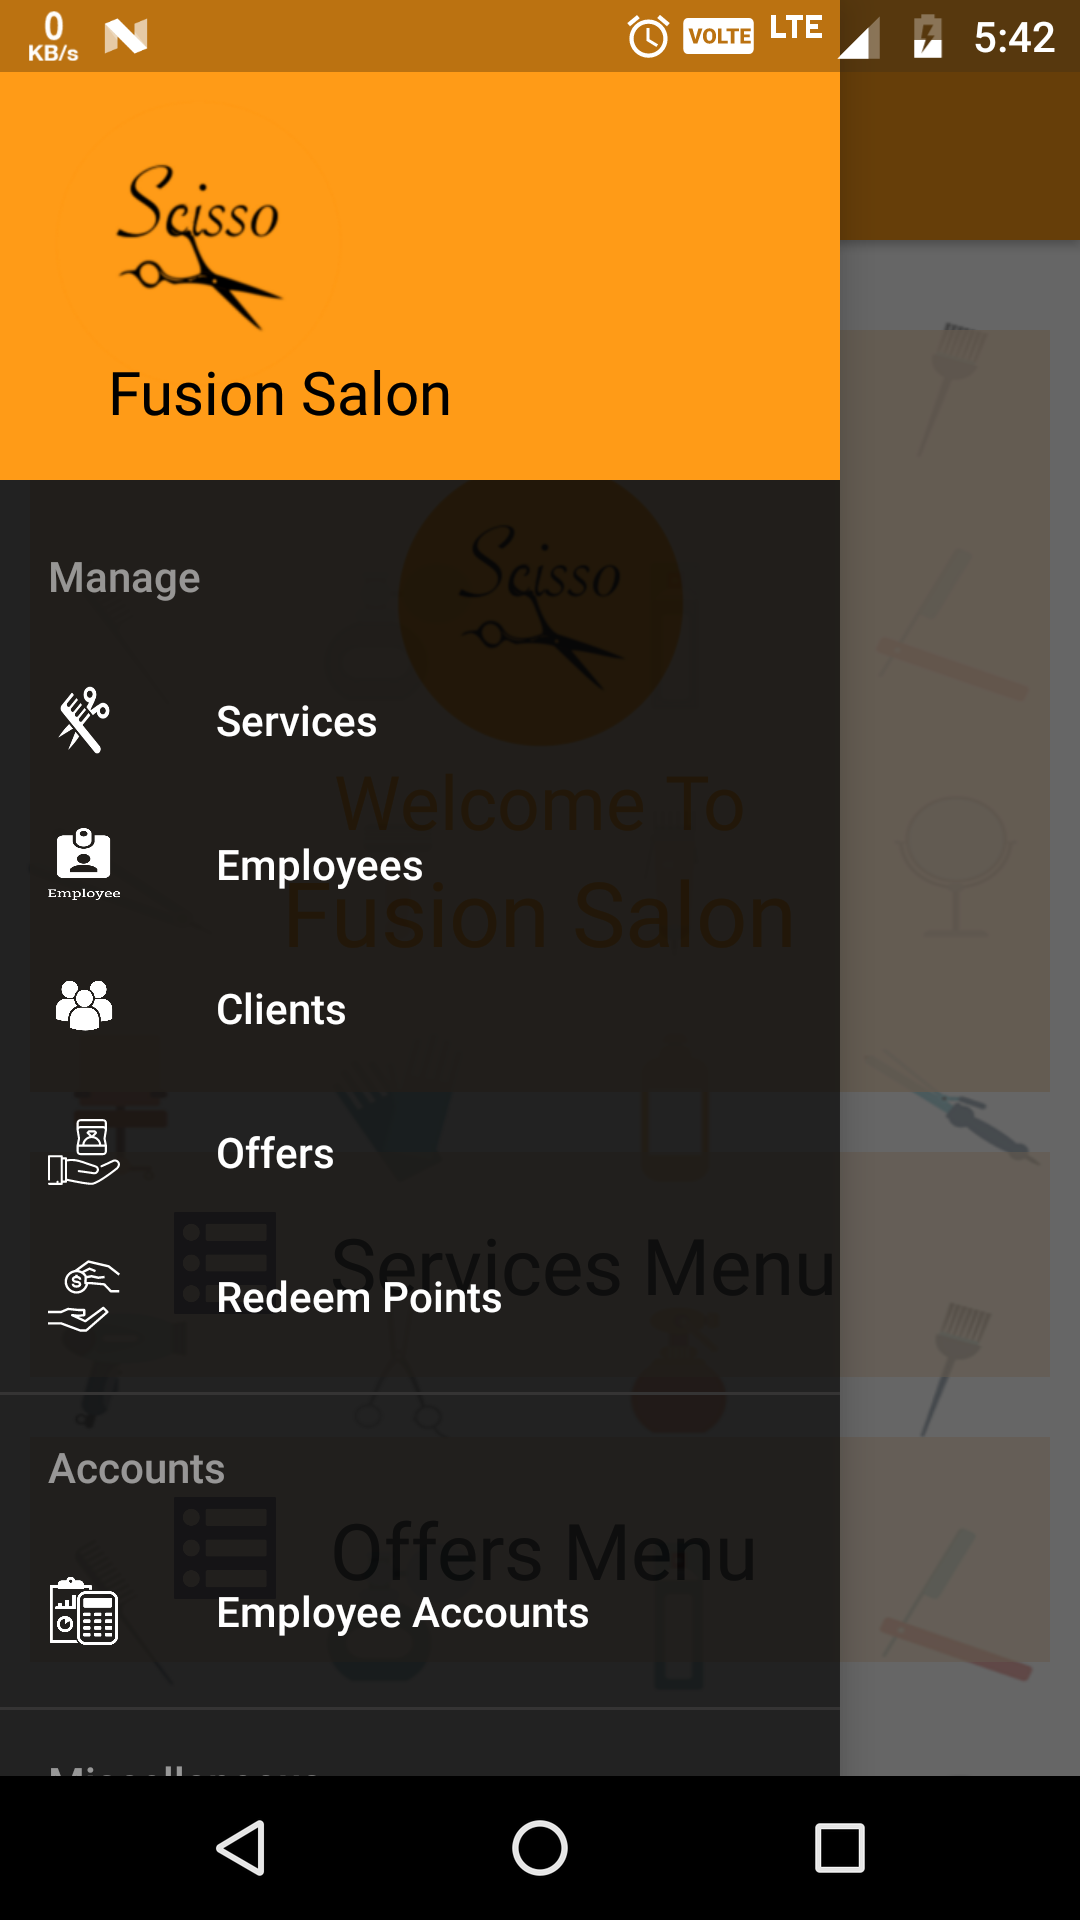
\includegraphics[width=0.7\linewidth]{NavigationView}
	\caption{Navigation View}
\end{figure}
\pagebreak

\\
\begin{figure}[h]
	\centering
	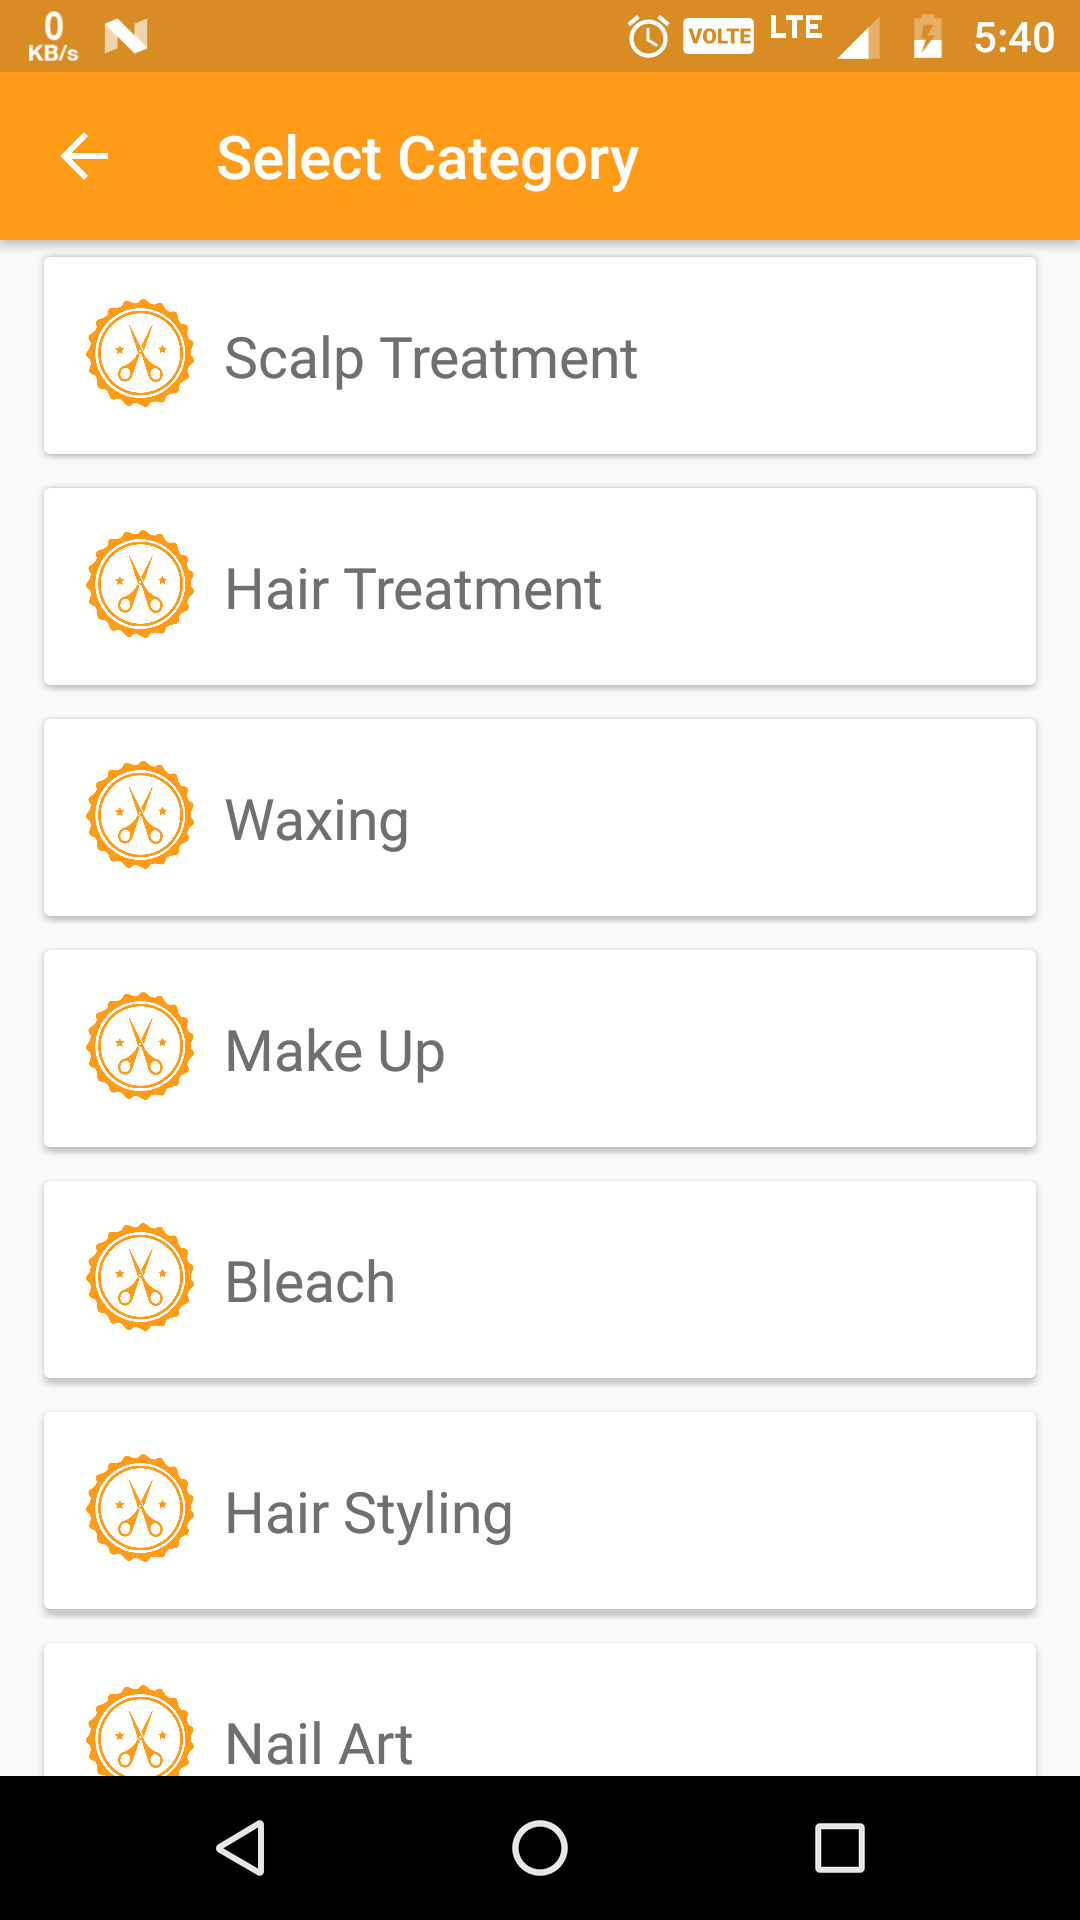
\includegraphics[width=0.7\linewidth]{SelectCategoryMenu}
	\caption{Select Category Menu}
\end{figure}
\pagebreak

\\
\begin{figure}[h]
	\centering
	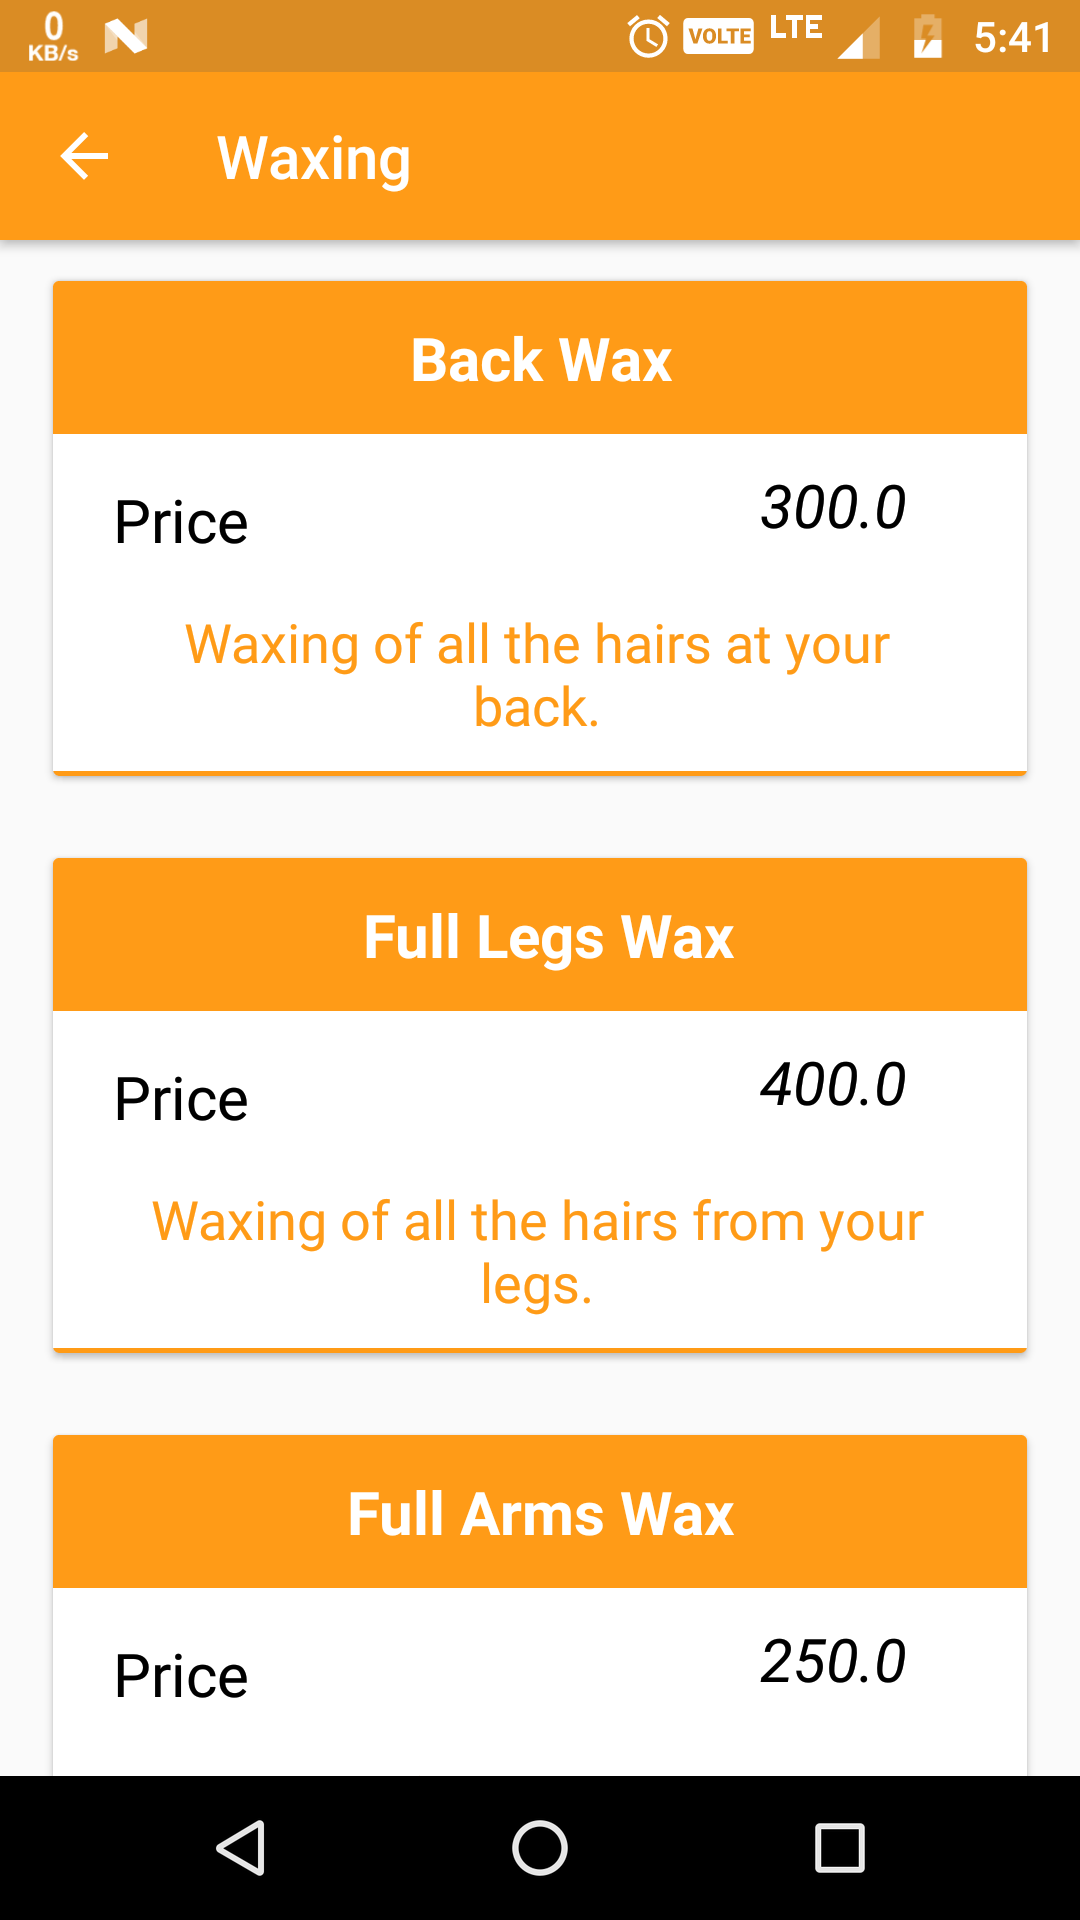
\includegraphics[width=0.7\linewidth]{ServiceListMenu}
	\caption{Service List Menu}
\end{figure}
\pagebreak

\\
\begin{figure}[h]
	\centering
	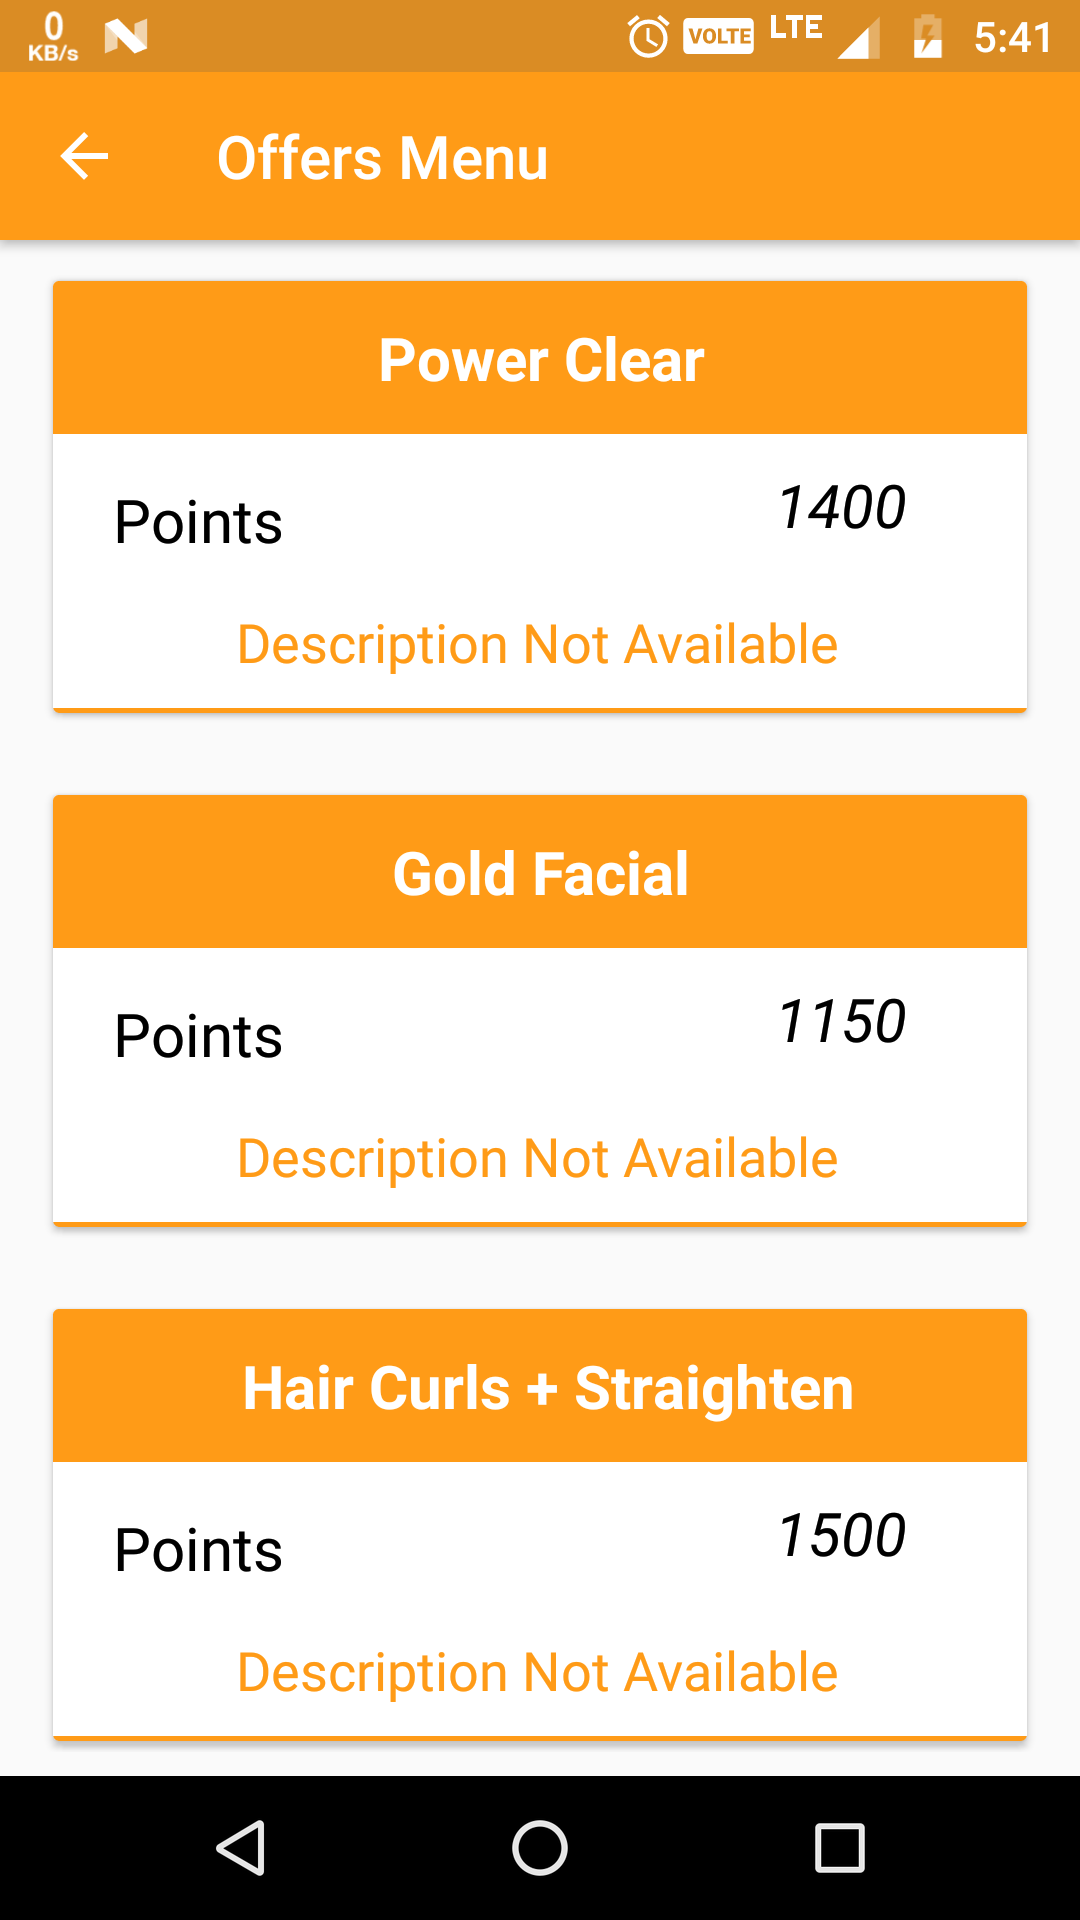
\includegraphics[width=0.7\linewidth]{OffersMenu}
	\caption{Offers Menu}
\end{figure}
\pagebreak

\\
\begin{figure}[h]
	\centering
	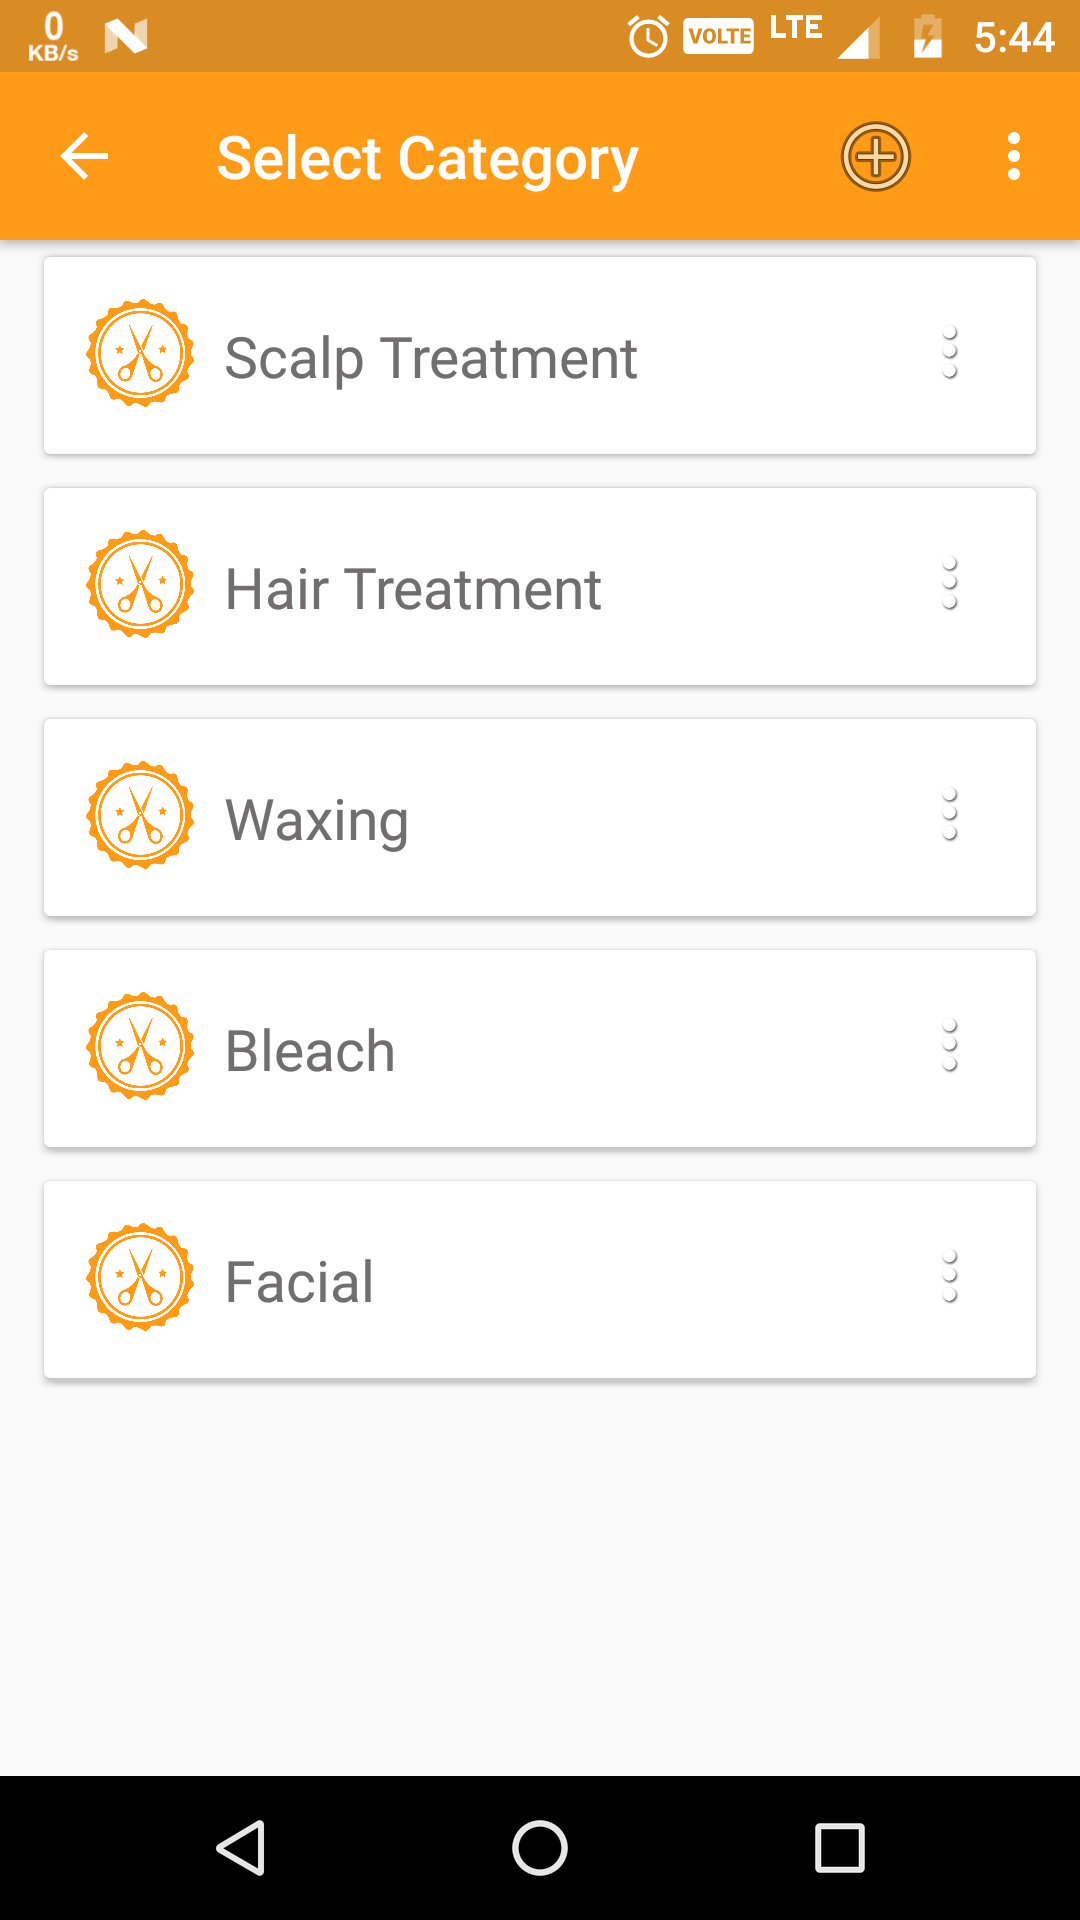
\includegraphics[width=0.7\linewidth]{EnabledCategories}
	\caption{Enabled Categories List}
\end{figure}
\pagebreak

\\
\begin{figure}[h]
	\centering
	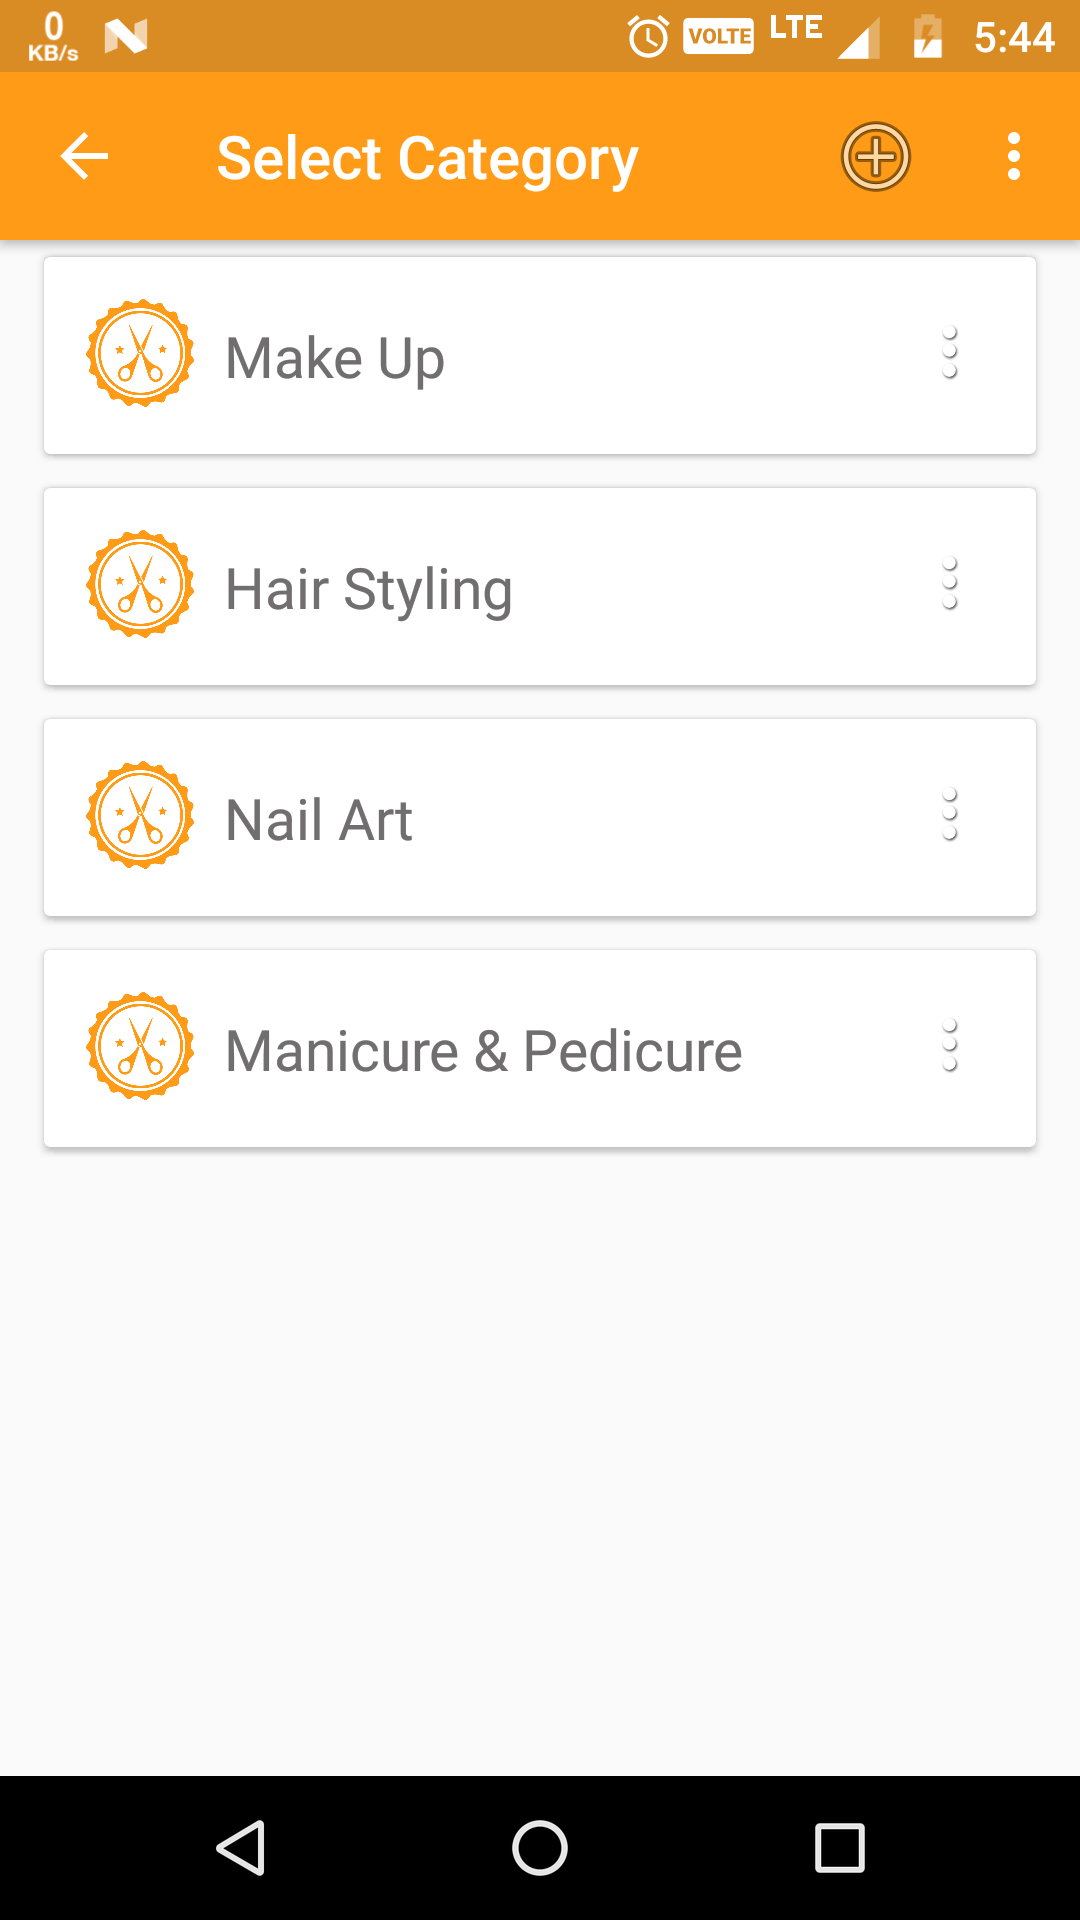
\includegraphics[width=0.7\linewidth]{DisablesCategories}
	\caption{Disabled Categories List}
\end{figure}
\pagebreak

\\
\begin{figure}[h]
	\centering
	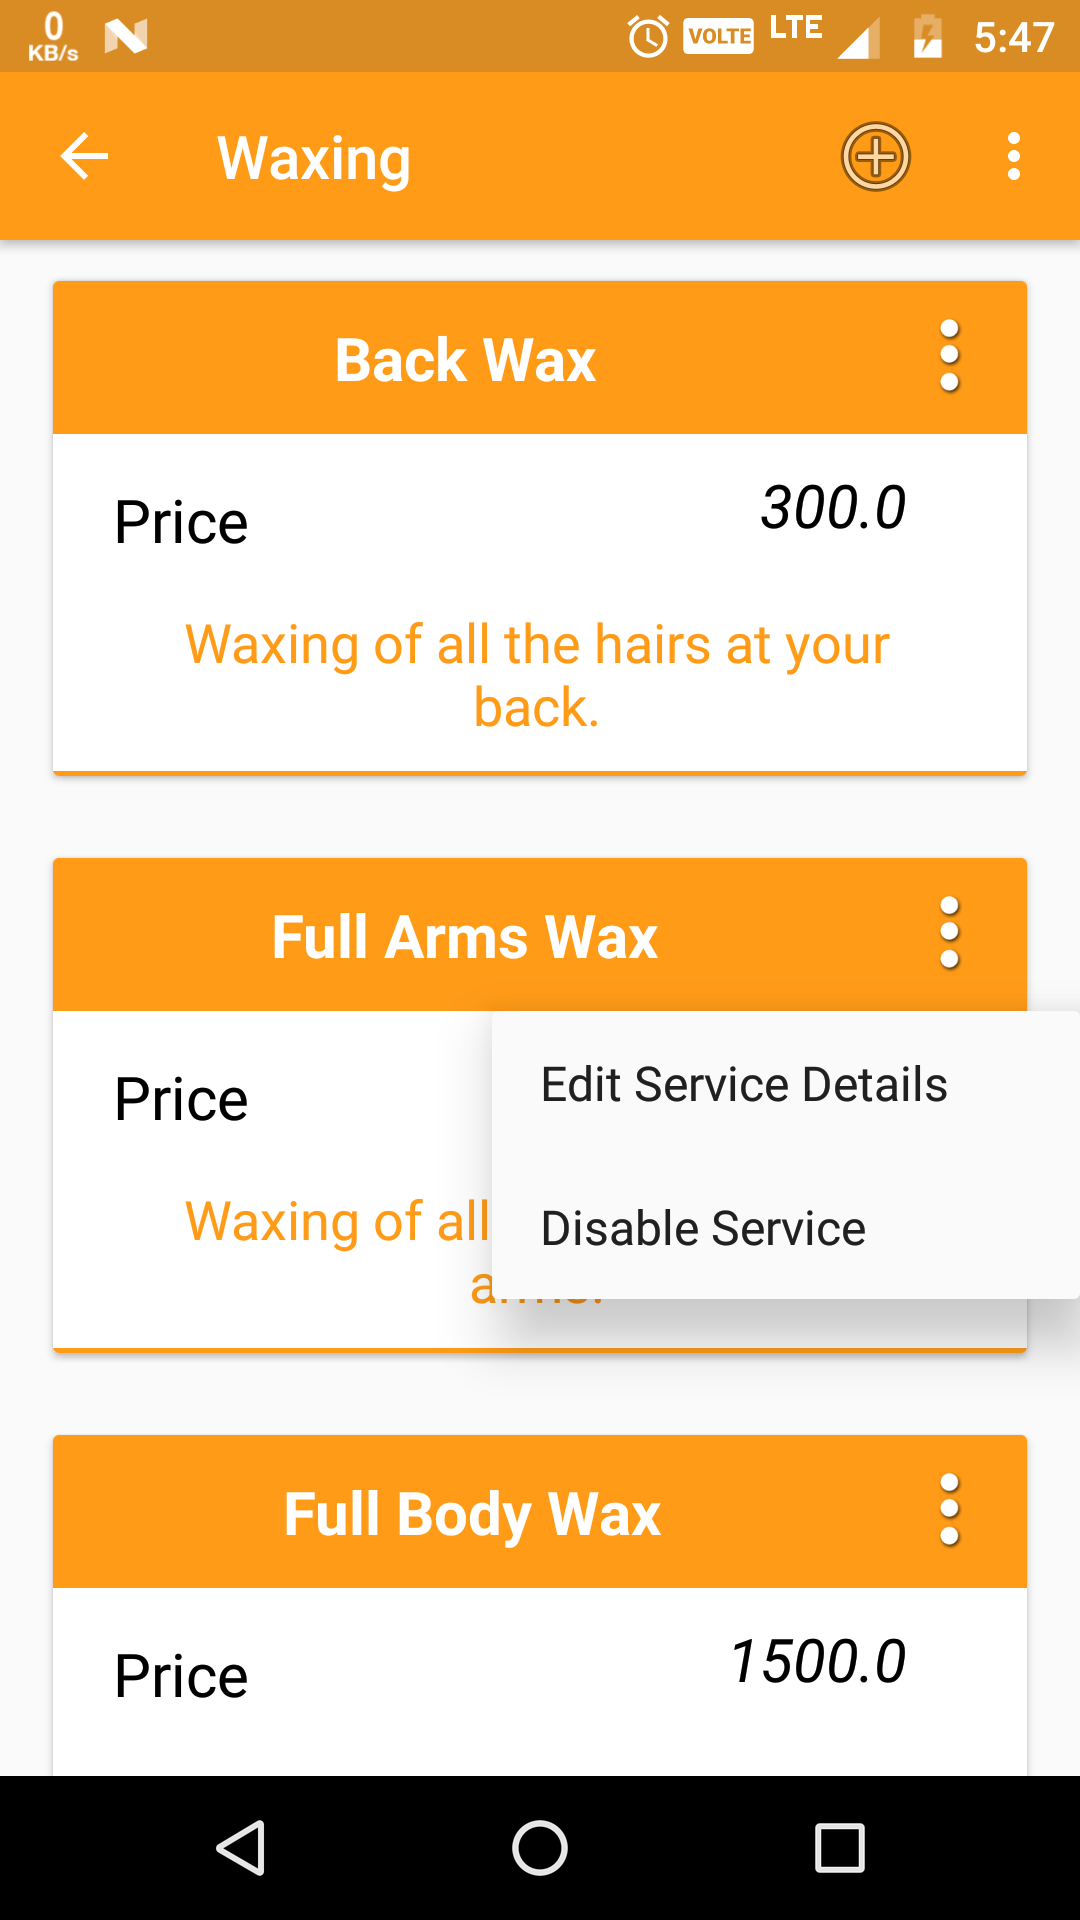
\includegraphics[width=0.7\linewidth]{EnabledServicesList}
	\caption{Enabled Services List}
\end{figure}
\pagebreak

\\
\begin{figure}[h]
	\centering
	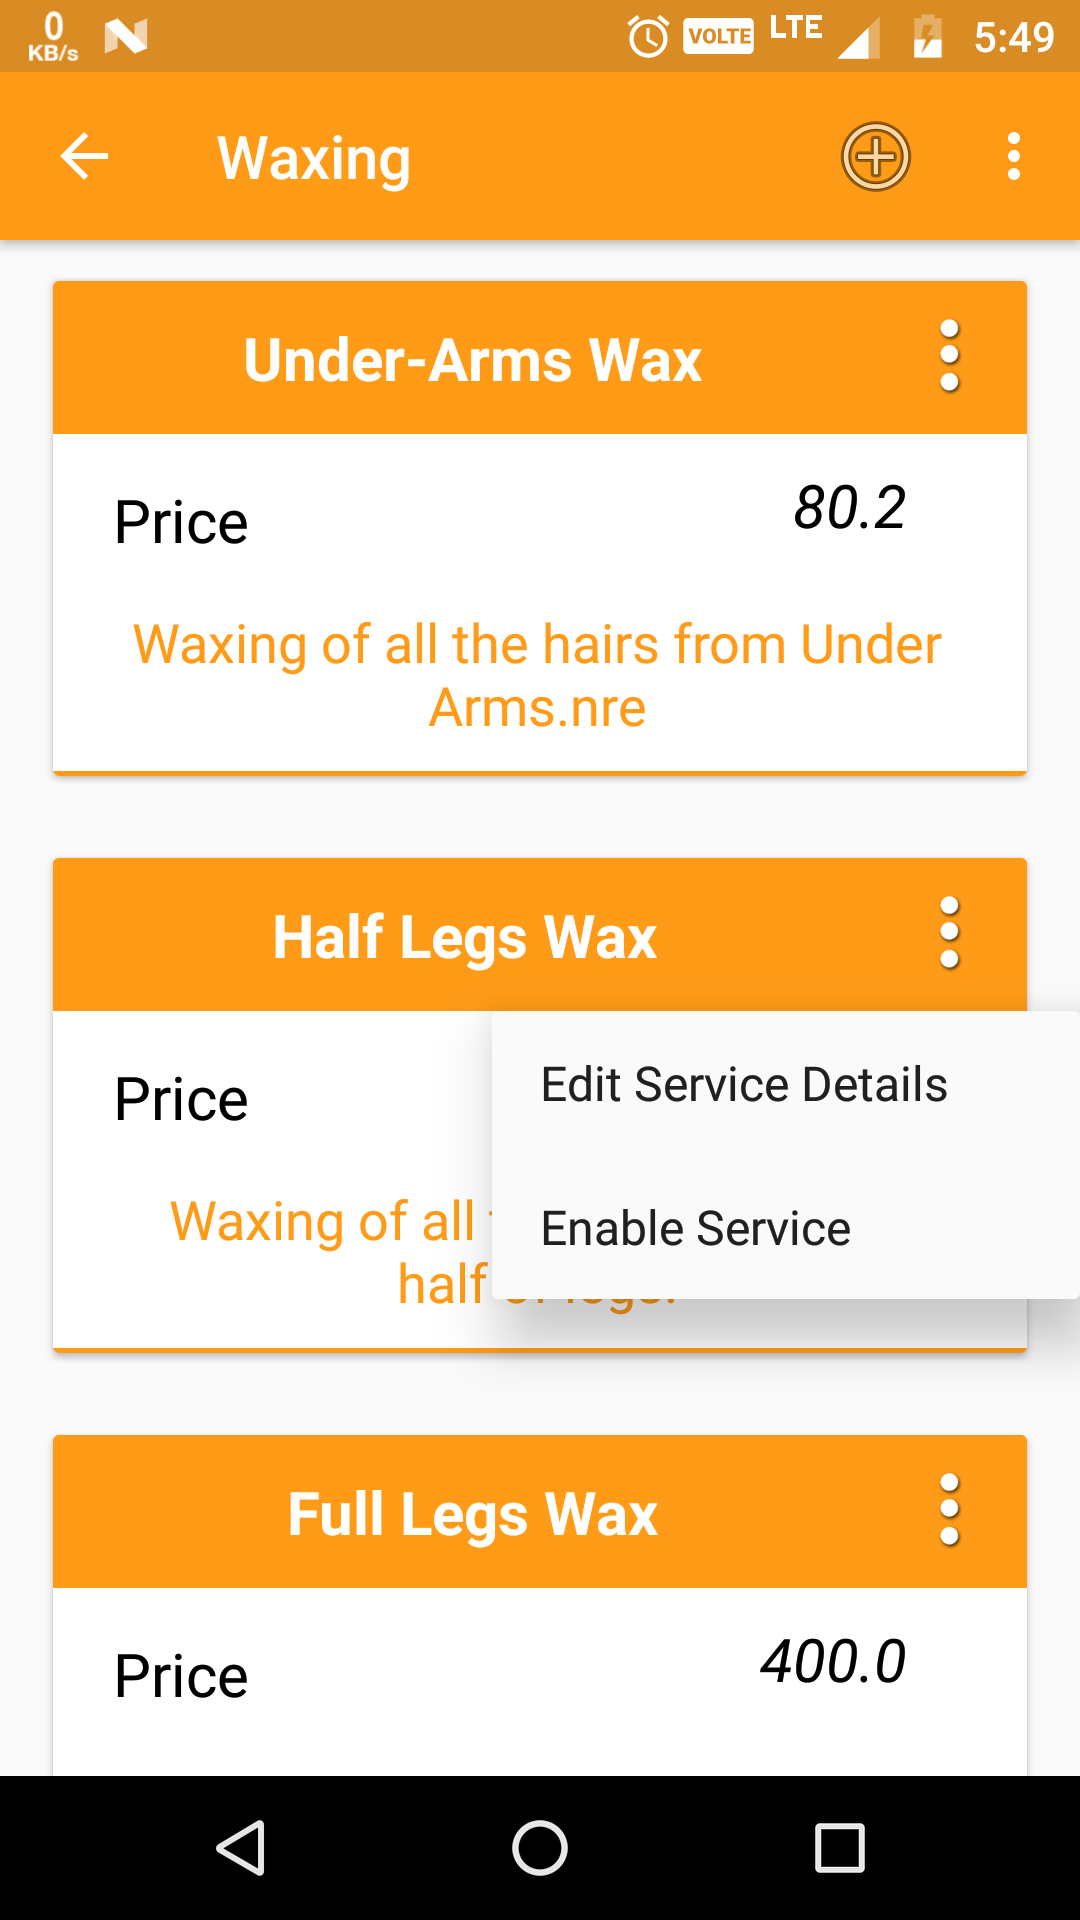
\includegraphics[width=0.7\linewidth]{DisabledServiceList}
	\caption{Disabled Services List}
\end{figure}
\pagebreak

\\
\begin{figure}[h]
	\centering
	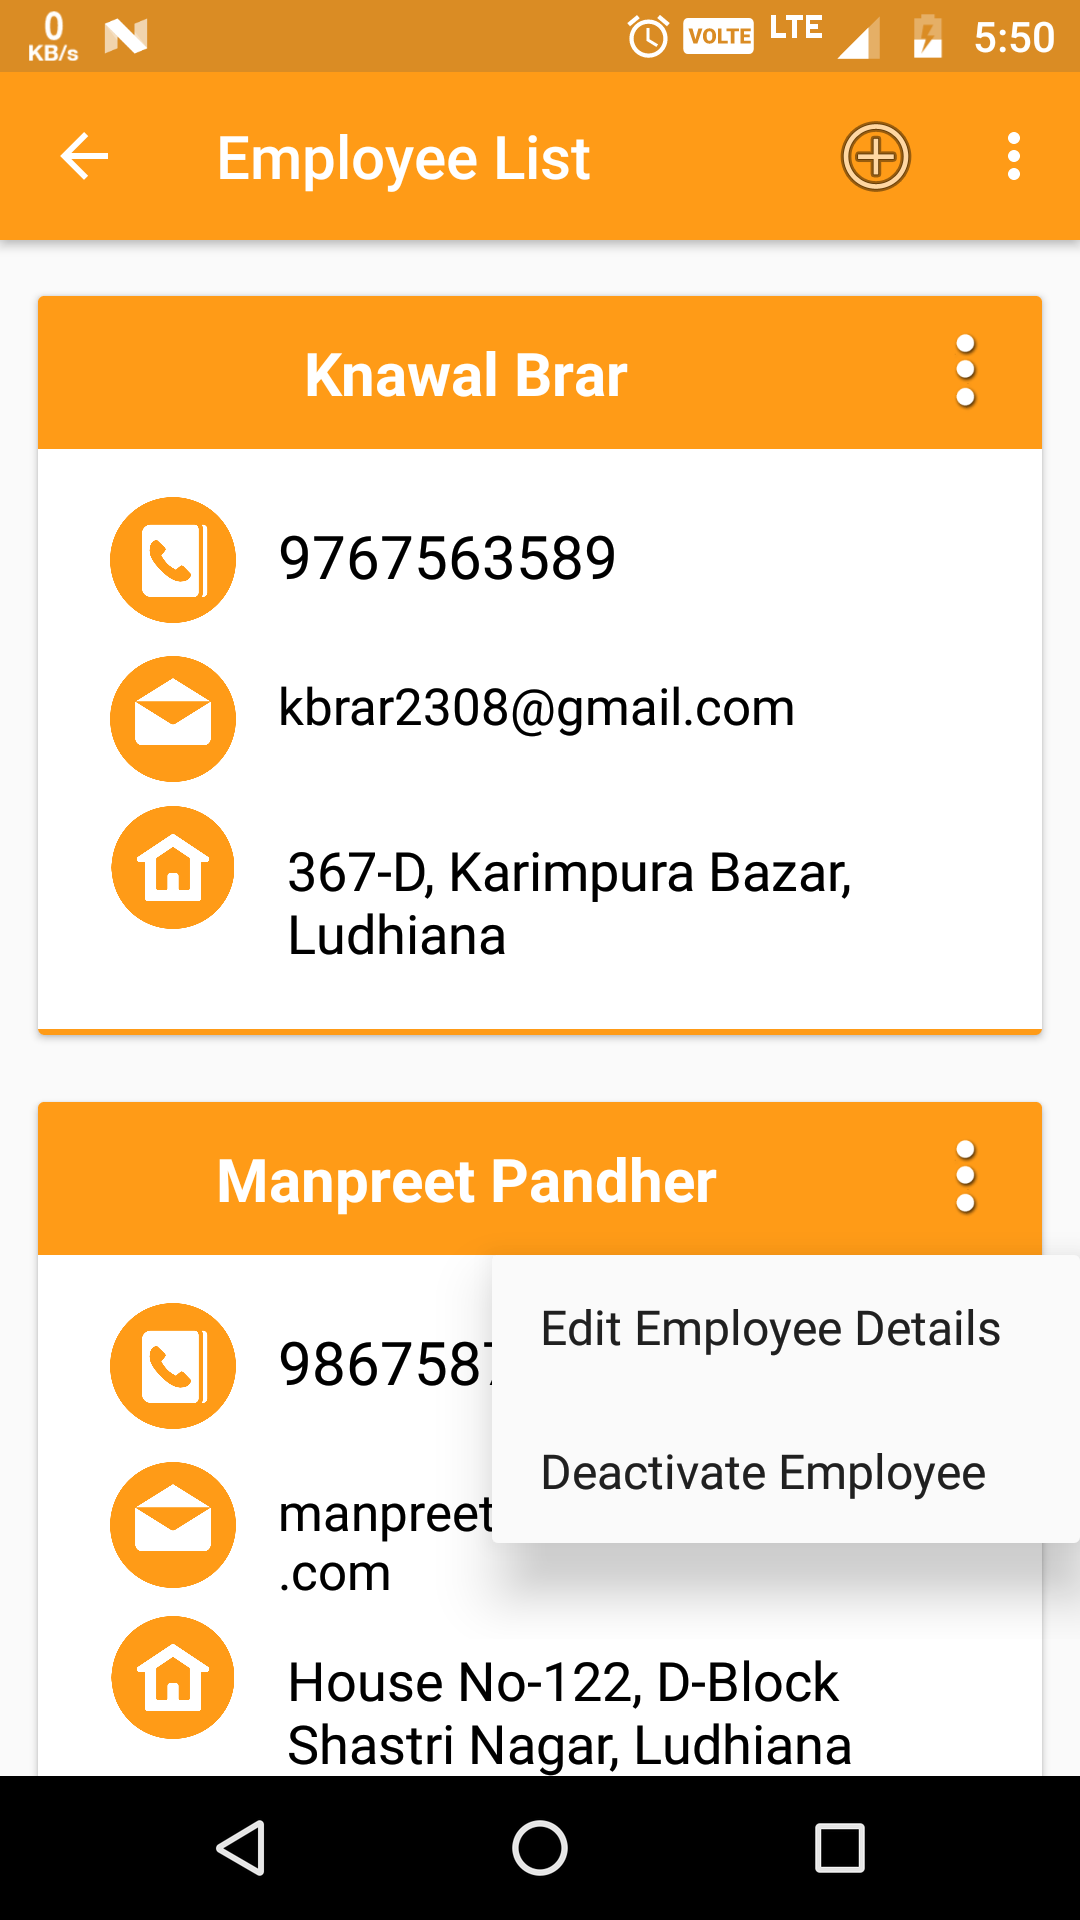
\includegraphics[width=0.7\linewidth]{ActiveEmployeeList}
	\caption{Active Employee List}
\end{figure}
\pagebreak

\\
\begin{figure}[h]
	\centering
	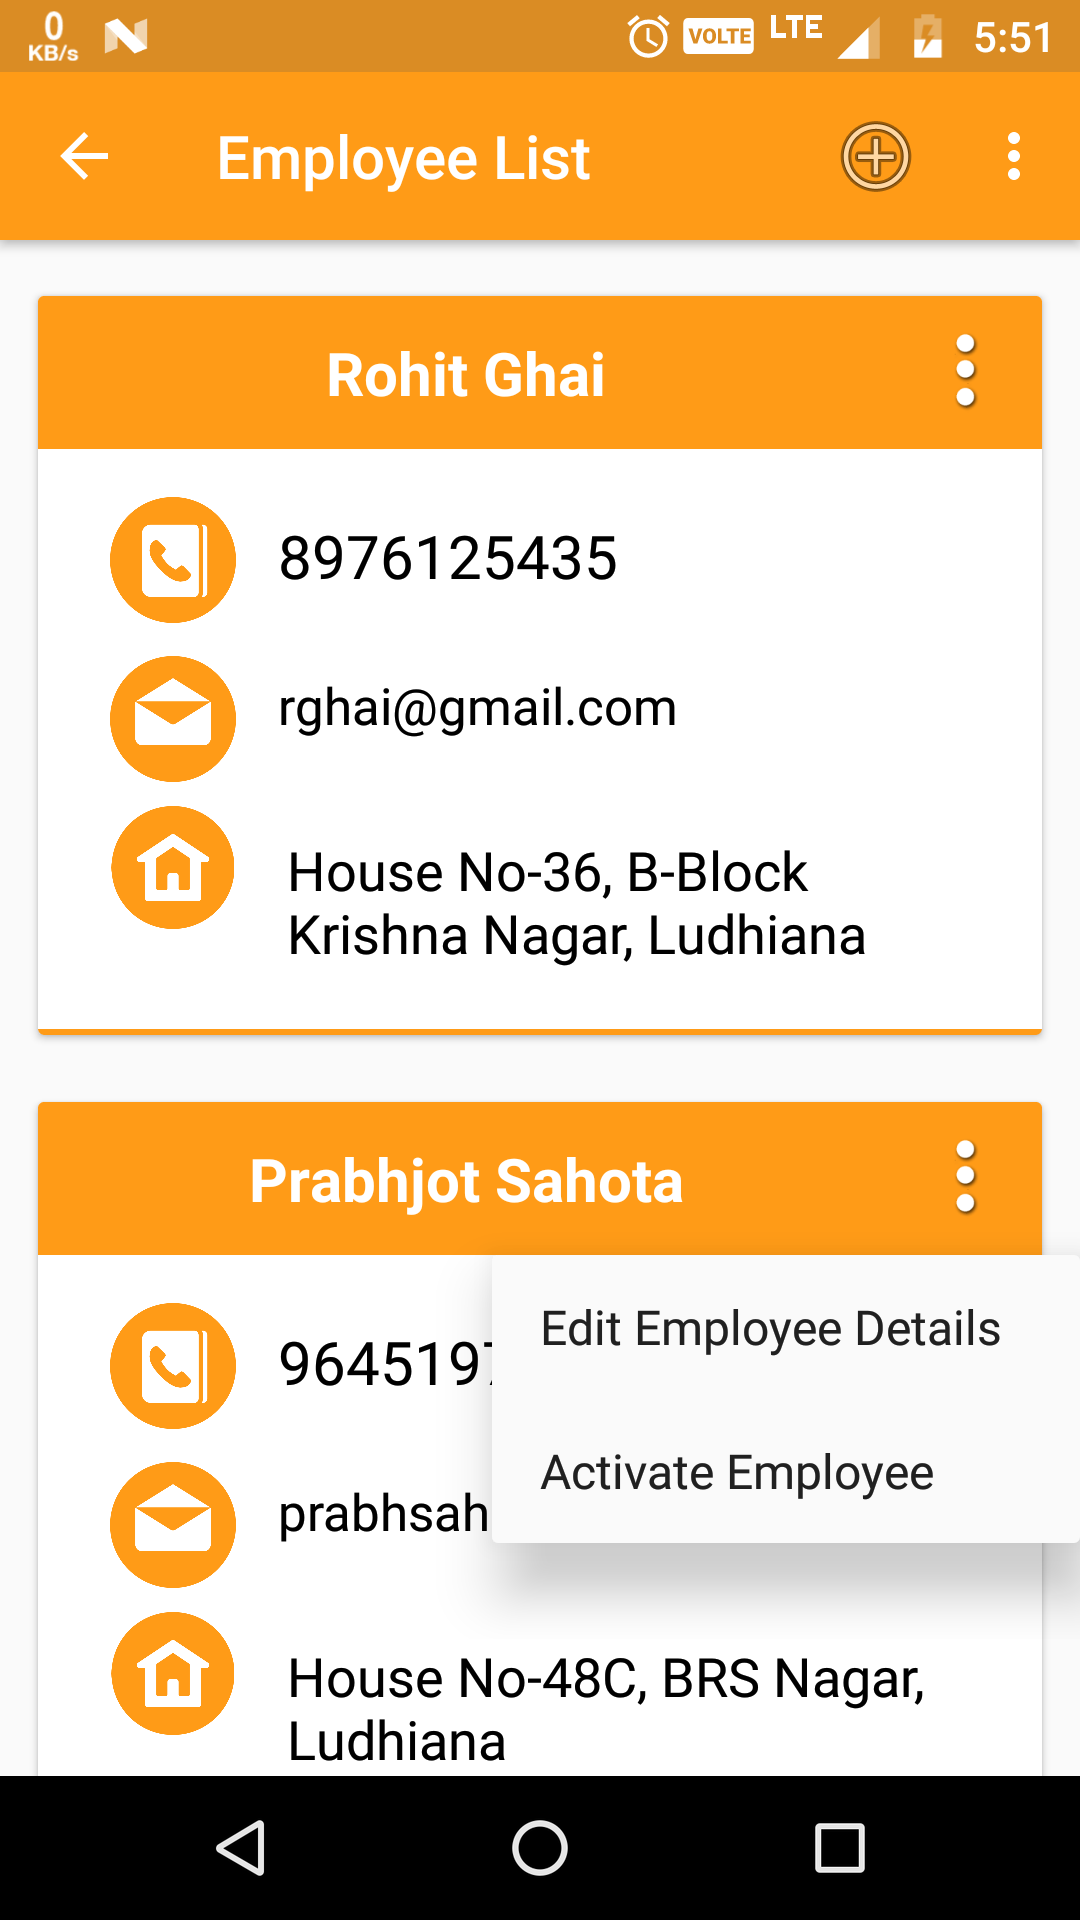
\includegraphics[width=0.7\linewidth]{DeactiveEmployeeList}
	\caption{Deactive Employee List}
\end{figure}
\pagebreak


\chapter{Refrences}\hrule
\label{Chapter:6}
% =====================================================================================================
\begin{enumerate}
	\item http://www.vogella.com/tutorials/android.html [accesed on 14/03/2018].
	\item https://www.tutorialspoint.com/android/ [accesed on 27/03/2018].
	\item https://developers.google.com/maps/documentation/android-api/marker [accesed on 03/04/2018].
	\item http://www.javatpoint.com/android-tutorial [accesed on 12/04/2018]
	\item http://www.vogella.com/tutorials/AndroidRecyclerView/article.html [accesed on \\13/04/2018].
	\item https://www.learnhowtoprogram.com/android/data-persistence/firebase-recycleradapter [accesed on 13/04/2018].
	\item 
	http://www.vogella.com/tutorials/AndroidTesting/article.html
	[accesed on 15/04/2018].
	\item 
	https://www.sharelatex.com/learn/Lists [accessed on 18/04/2018].
	\pagebreak
\end{enumerate}